\startchapter{Intelligent Meter Placement}
\label{chap:meterPlacement}
In this chapter, we solve the meter placement problem using entropy-based measurements and Bayesian network models to identify the most suitable power links for power meter placement. To ease understanding, we list the nomenclature used in this chapter first. 

\section{Introduction/Motivation}
Monitoring power quality is not an easy task. Since the power quality measurement devices~\cite{schneider_meter} are expensive, it is financially impractical to monitor every segment of a power network. The overhead of interconnecting these power meters and developing the power management system further increases the cost. Therefore, we need to intelligently place power quality meters on selected power links to reduce the uncertainty of power quality estimation on unmonitored links in the power grid. The following core challenge needs to address: given a fixed number of available power meters, which grid segments should be selected for monitoring such that power quality can be inferred in the remaining unmonitored segments of the network.

As the first step to tackle the above challenge, the probabilistic calculation of power quality values on unmonitored links requires the behavior (latent feature) of each device to be known. We represent the latent feature of a device as a transition function which is usually estimated through physical modeling or through the assessment of historical power monitoring data. Using a real power quality dataset, we show that historical data can be used to capture the latent features of a device.

With devices' latent features captured, we in the second step introduce a network model which represents the smart microgrid as a data-driven network. In analogy, we represent the electrical components as network nodes, power links as data links, and flow of power as data flow on the links. This problem transformation significantly simplifies the complexity of the power network; it also presents the opportunity to use the well-investigated network monitoring and data estimation algorithms to solve the network quality monitoring problem.

Finally, we solve the intelligent meter placement problem by proposing an iterative approach for identifying network segments suitable for power meter placement. During each iteration of the algorithm we identify in a greedy manner the network segment whose power quality is most unpredictable given the meters placed so far. We then place the next power meter at that location. In this chapter, we make the following contributions. 
\begin{enumerate}
	\item A network model for power quality estimation, based on the device latent features that are learned from a real-world dataset, 
	\item An intelligent entropy-based algorithm and a Bayesian network-based approach to solve the meter placement problem.
	\item Formulate the problem of estimating the number of required power meters to achieve the desired level of reliability as an optimization problem.
\end{enumerate}

\section{Related Work}
This work is related to four categories of research and development: power quality classification, power reliability, power quality improvement/estimation, and meter placement. We summarize the relevant literature in these categorize in Section~\ref{sec:related_work}. We re-iterate the three main differences between the existing PMU placement algorithms and our proposed algorithm as follows.

\begin{enumerate}
\item We focus on distribution networks at the enterprise level (e.g., a university campus).
\item Our method is data driven and is based on statistical machine learning method.
\item The existing PMU placement algorithms address the problem of estimating network states and do not consider power quality estimation explicitly.
\end{enumerate}

\section{Meter Placement Problem Formulation}
Before we formally illustrate our proposed algorithms for the deployment of power meters in the electric power grid, we detail our assumptions about the structure and function of the power grid network as follows:

\begin{enumerate}
\item \emph{The power grid network is a tree-structured network where the electric current flows from root node to the child nodes.}
Note that this is a 
reasonable assumption at any particular instance in time. While enterprise-level power grids used in places such as hospitals and data centers often have two utility feeds available as well as an independent emergency power source, only one power source is typically used at one time. See the IEEE Gold Book~\cite{goldbook} for further information on recommended practices in the design of critical power systems. 

\item \emph{The probability mass function (pmf) of power quality values at the input link to the root node is known.} In other words, the distribution of power quality at the input to the network, usually the utility feed, is known.
This is also a reasonable assumption, since electrical utilities typically report on indices such as SARFI which is essentially a count of the number of times the magnitude and duration falls below a threshold.  
Furthermore, there are often independent bodies that gather statistics on power delivery service reliability that can also be incorporated into an estimate of power quality distribution~\cite{chowdhury2004reliability}. 

\item \emph{The power quality transfer function $f(d)$ is known for every device $d$.}  
A device-specific power quality transfer function could be estimated for specific models of electrical components 
through physical modeling or through the assessment of historical power monitoring data. 
Given a reasonable initial estimate, 
the transfer functions could be further refined through online learning techniques~\cite{catherine_pri}. 
\end{enumerate}

Given the assumptions listed above we can define a power meter placement algorithm as a process that takes as 
an input: the topology of the smart grid, an \textit{a priori} estimate of the feed \emph{pmf}, the power quality transfer function for each component, and the total number of meters $M$. The output of the algorithm is a set of $L$ locations for deploying power meters. 

\section{Meter Placement Algorithms}
\subsection{A Simple Entropy-based Approach}
\label{sec:simpleH}
We propose to deployed the power quality meters on network segments where the power quality values are most uncertain. We measure the uncertainty of power quality on a link using Shannon's entropy measure. Therefore, the entropy formula to measure uncertainty at the output link of a device $d$ becomes
\[H(d) = H(l_{o}^{(d)}) = -\sum_{i=1}^n p_{c_i}^{(d)} \log p_{c_i}^{(d)},\]
where $p_{c_i}^{(d)}$ is the probability of power quality $c_i$ at the output link of device $d$.

\begin{algorithm}[!p]
\setstretch{1.5}
\vspace{0.2cm}
\KwIn{distribution function of input link to device 1 i.e., $f_x^{(0)}$, \\transfer function $f(d)$, and number of power meters $M$.}
\KwOut{$L$ (list of devices to be selected for meter placement)}
\Begin{
   \ForEach {(device $d$)}{
      $\hat d \leftarrow getParent(d);$ \\
      /* Note that device 1 (root of the tree) has no parent \\ i.e., \emph{getParent(1) = 0} and $f_x(0)$ is given */\\
      $f_x(d) \leftarrow f_x(\hat d) \times f(d)$; \\
      $H(d) \leftarrow - \sum_{i=1}^n p_{c_i}^{(d)} \log p_{c_i}^{(d)};$\\
      /* where $p_{c_i}^{(d)}$ is the $i^{th}$ component of $f_x(d)$ vector */
   }
/* get $N$ high entropy devices in vector $H$ */\\
$L \leftarrow getHighEntopyDevices(H, N);$
}

\vspace{0.2cm}\caption{A Simple Entropy-based Algorithm}\vspace{0.2cm} \label{algo-1}
\end{algorithm}

In order to calculate $H(d)$, we need to know the power quality distribution function of link $l_{o}^{(d)}$. Starting from the root node of the tree-structured network, we traverse all the nodes (devices) in level-order fashion to calculate the distribution function $f_{x}(d)$ as $f_{x}(d) = f_x(\hat d) \times f(d)$. After calculating $f_{x}(d) = [p_{c_1}^{(d)} \ p_{c_2}^{(d)} \ \dots \ p_{c_n}^{(d)}]$ where $p_y(d) = \sum_{x=1}^n p_x^{(d)} \times p_{c_y \mid c_x}^{(d)} \ \forall \ y = 1,2,\dots,n$.

The detail of our entropy-based meter placement algorithm is shown as Algorithm~\ref{algo-1} where the power meters are placed on network segments having maximum uncertainty in power quality values. This simple algorithm is fast and useful when there is negligible impact of a link on any other link in the network. For instance, if a node always produces a power quality $c_1$ as output irrespective of the input quality (a stabilizer). Nevertheless, in most cases the network links are dependent on each other. Therefore, we need to consider the link dependency while calculating the uncertainty of a link, i.e., a meter reduces the entropy not only on the measured link, but also on other links in the network. Further, based on our initial tests with the simple Algorithm~\ref{algo-1}, we conclude that it may create a poor allocation scheme for some cases. In the remainder of this section, we further investigate the problem and propose more robust methods to address the power meter placement problem. 

\subsection{Bayesian Network-based Approach}
\label{sec:predict} 
This section describes a Bayesian network-based algorithm for selecting locations for placing power meters in a power grid. The approach uses Monte Carlo sampling and probabilistic inference approaches to identify locations in the power grid which exhibit unpredictable power quality events.

The problem is inherently challenging as the information received from a power meter flows not only the forward direction from the root nodes toward the leaf nodes, but also in reverse or upstream direction toward the root node (utility main) and back to all other nodes in the network. 

To tackle the above challenge, we cast the problem as a Bayesian network and model the power grid using a factor graph. Several message passing algorithms could be used to help us determine the optimal meter placement. We chose the belief propagation or sum-product algorithm~\cite{pearl1988probabilistic}, since it is well understood and has been shown to work for general topologies~\cite{yedidia2001generalized} including tree networks.

\subsubsection{MC Event Sampling}
Given the transition function $f(d)$, we use a Monte Carlo (MC) method to obtain a set of $K$ samples at each node $d$. We first compute a \emph{pmf} $f_x{(d)}$ for each node $d$ using its transition function $f(d)$ and the \emph{pmf} of its parent node $\widehat{d}$ as $f_x(d) = f(d) \times f_x(\widehat{d})$. Then, at each time slot $i \in \{1\ldots K\}$, we draw a sample $c_{i}^{(d)}$ from $f_x(d)$ at each node $d$. We repeat this at each node of the tree starting from the root and ending at the leaves. The result is a set of $K$ simulated samples $C_{i}=\{c_{i}^{(1)},c_{i}^{(2)},\ldots,c_{i}^{(N)}\}$ for each of the $N$ links in the power network. 

\begin{figure}[!p]
\vspace{1cm}
\centering
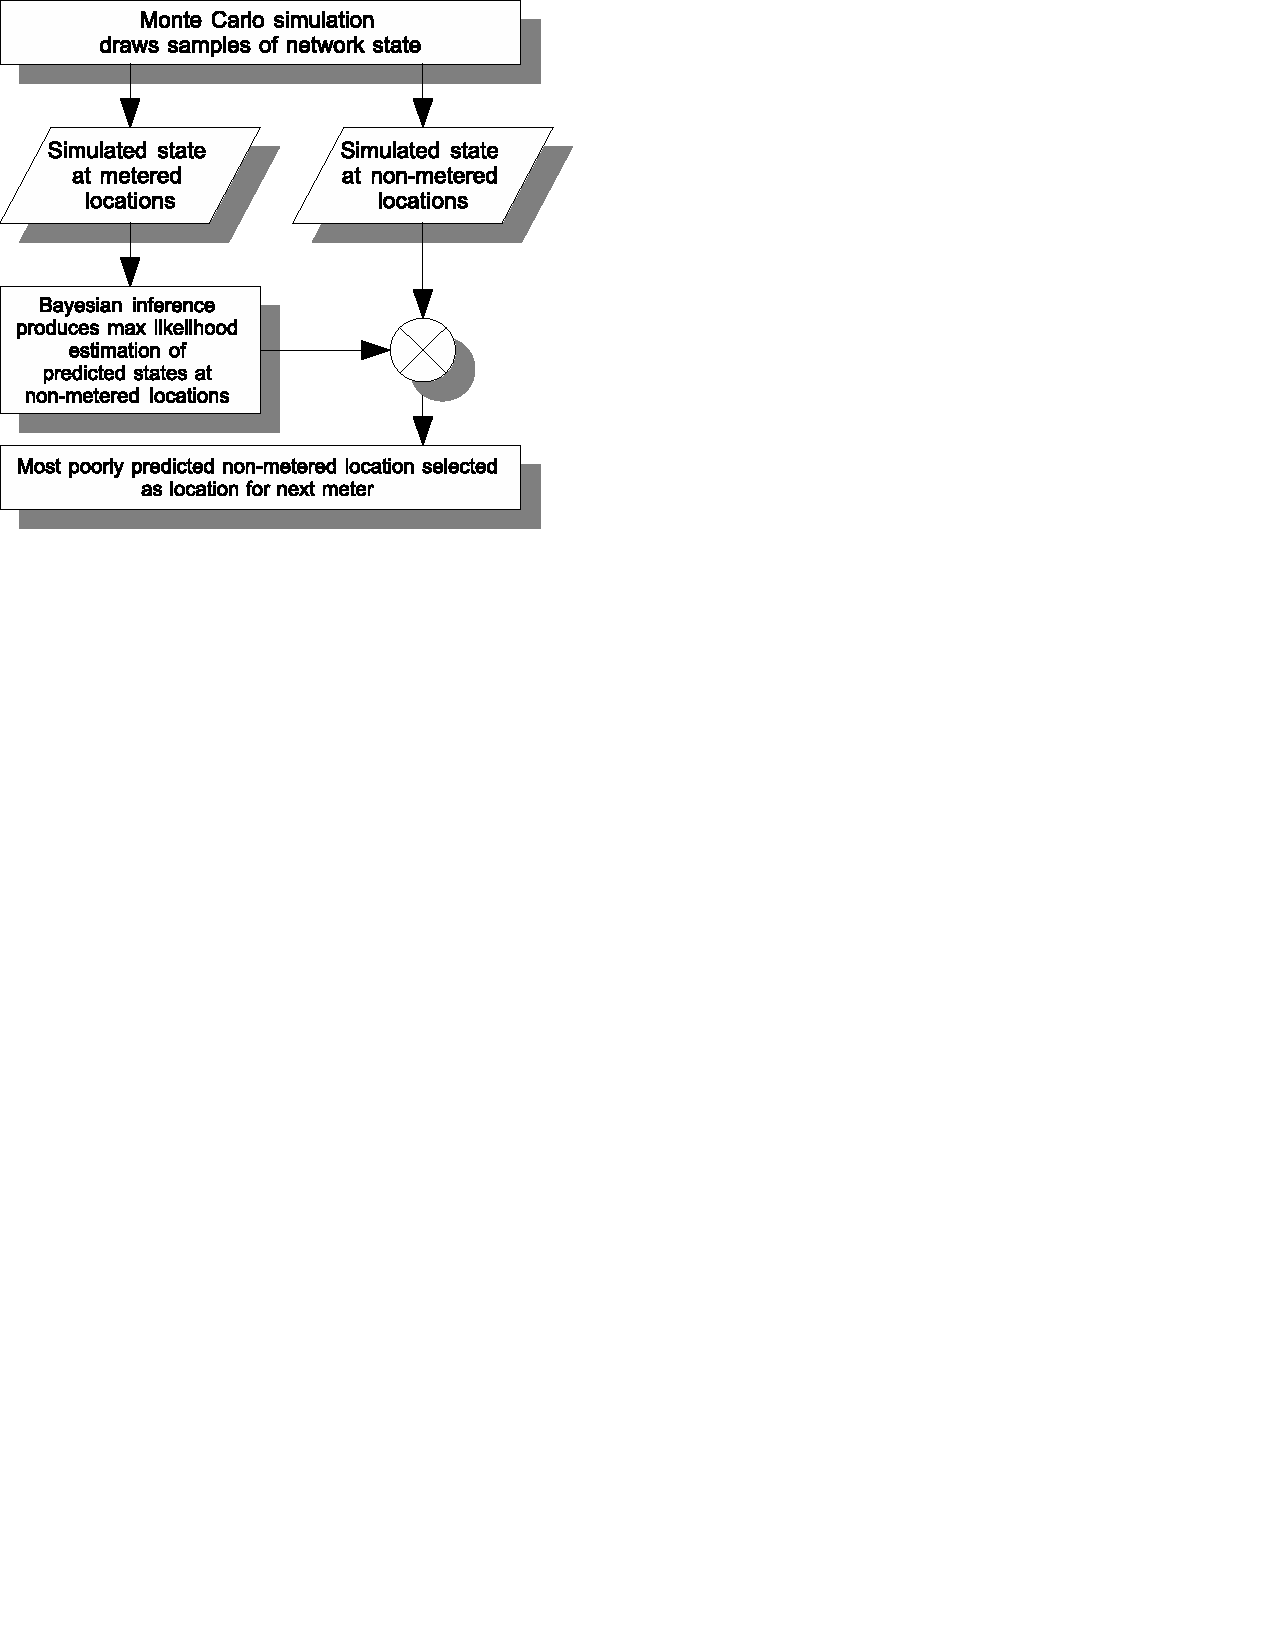
\includegraphics[width=0.7\columnwidth]{flowchart_worst_predicted_error}
\vspace{0.5cm}
\caption{Data flow diagram of meter selection process during a single iteration of the greedy algorithm.}
\label{flowchart}
\end{figure}

\begin{figure}[!p]
\centering
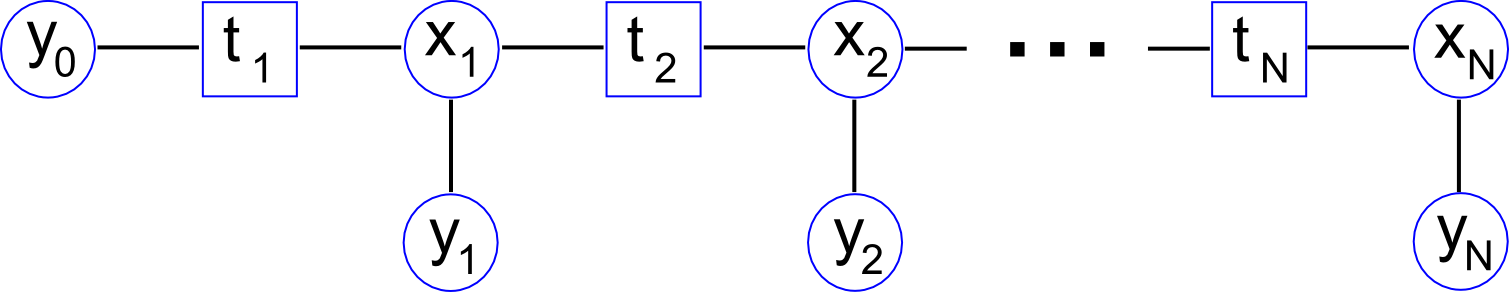
\includegraphics[width=0.9\columnwidth]{factorgraph}
\vspace{0.5cm}
\caption{Power network modeled as a factor graph}
\label{factorgraph}
\vspace{2cm}
\end{figure}

\subsubsection{Event Inference using Belief Propagation}
The samples obtained by the MC simulation of power quality propagation contain consistent sets of power quality values at both metered and unmetered locations. We use Bayesian inference to infer the power quality at unmetered locations as a function of the  simulated values observed at the metered locations and compare the resulting predictions to the simulated value seen at the unmetered locations. This process gives a relative indication of the predictive strength on each link of the network. Figure~\ref{flowchart} shows a high-level description of this process.

\begin{algorithm}[!p]
\vspace{0.2cm}
\setstretch{1.2}
\KwIn{The topology $T$ of the power grid,
the input feed to first device $f_x{(0)}$, 
transition functions $f(d)$,
maximum number of meters $M_{max}$,
maximum uncertainty to allow $\delta_{max}$,   
and the number of Monte Carlo samples $K$ to draw.} 
\KwOut{$L$ (list of links to be selected for meter placement)}
\Begin{
$M \leftarrow 0;$ $\delta_{curr} \leftarrow \delta_{max};$ \\
   \While {($M < M_{max}\ and \ \delta_{curr} \geq \delta_{max}$)}{
		  $\epsilon_l \leftarrow 0$, $\forall$ links $l \in T$;\\
		  /* $\epsilon_l$ is prediction error at link $l$ */\\  
      \ForEach {(Monte Carlo Sample $k$)} {
				%$x = ( x_m \cup \hat x_m ) \leftarrow $ sample of instantaneous network state;\\
				$L \leftarrow$ set of metered links $\in$ $T$; \\
				$L' \leftarrow$ set of unmetered links $\in$ $T$;\\
				$\widehat C_k\leftarrow$ predictPowerQuality($L', L, T$);\\
				 /* $\widehat C_k$ is the $k^{th}$ set of predicted power quality values while $C_k$ is the $k^{th}$ set of sampled values at all links*/\\  
      	\ForEach {(link $l \in L'$)} {
					\If { $\widehat c_k^{(l)} \neq c_k^{(l)}$ } { 
						$\epsilon_l \leftarrow \epsilon_l + \frac{1}{K}$; /* add $\frac{1}{K}$ to predicted error */
					}
				}
      }
      $selectedLink \leftarrow \max(\mathcal{E}).position$; \\ /* $\mathcal{E} = \{\epsilon_l\}$  i.e., set of $\epsilon_l$ $\forall$ $l$ */ \\
      $L$.add($selectedLink$);\\
      $\delta_{curr} \leftarrow \max(\mathcal{E});$ $M \leftarrow M + 1;$
   }
}
\BlankLine
$function$ predictPowerQuality($L', L, T$) : $C_k$\\
\Begin{
	init pmf $\Psi = \{ \psi_l \}, \forall$ links $l \in T$;\\
	$\Psi' \leftarrow$ BeliefPropogation given evidence $L$\\
  \ForEach {( link $l \in L'$)} {
		$c_k^{(l)} \leftarrow$ max probability power quality class inferred in $\psi_l'$;
	}
	$C_k = \{c_k^{(l)} \}$; 
}
\caption{Monte Carlo Predicted Error Algorithm} \label{alg-3}
\end{algorithm}

\noindent \\
To do the prediction, we first model the power network as a factor graph (Figure \ref{factorgraph}) and then use belief propagation to find the inferred values of power quality at the output of each node using the (simulated) evidence obtained from the power meters. The factor graph has conditional probability nodes $t$, equality nodes $x$, and evidence nodes $y$. The $t$ nodes represent actual electrical devices with a known transition function. The $x$ nodes represent wired connections on our network for which we have already obtained a set of samples using MC sampling. These nodes are constrained so that all edges connected to them are equal. The $y$ nodes represent locations where a power meter could be placed. The unmetered nodes are initialized to a uniform \emph{pmf} and the metered nodes are set to a trivial \emph{pmf} with a probability of $1$ at the true power quality event and $0$ everywhere else. 

For each time slot $t_{i}$ we infer the maximum likelihood power
quality event that would appear at each node given the current meter
configuration. We then estimate the error rate for each node in the
network. If the inferred event differs from the event given by the
MC sample we add $1/K$ for that sample. At each round of the algorithm
we greedily choose to place a meter at the node with the highest error
rate. We terminate the algorithm when all meters have been placed.

The number of required power quality meters could be determined based on: 1) the available financial budget, and 2) the desired estimation accuracy. We consider both aspects. The proposed algorithms keep placing meters until either the maximum meter limit is exhausted or the desired estimation accuracy is achieved. The estimation accuracy is captured by the certainty of PQ values on network segments. See Algorithm \ref{alg-3} and Figure \ref{flowchart} for further details.

\subsection{Conditional Entropy (CE)-based Approach}
Since the PQ values on network segments are dependent on each other, we exploit the idea of conditional entropy to propose another new algorithm. Further, this approach is much faster than the Bayesian network (BN)-based approach without compromising the accuracy. The idea here is to install each power meter under consideration on a network segment $i$ which results in maximum reduction in overall network entropy. We consider all possible placement points for every meter to be placed and choose a link which reduce the network entropy at maximum. Note that a reduction in network entropy is the sum of entropy reduction on the underlying link $i$ and all other links whose entropy is minimized/reduced in effect of meter placement on a segment $i$. The one time matrix multiplications in this approach are much faster than our previous requirement of re-sampling the network state after every possible meter placement.

The CE-based algorithm is efficient and scalable to large scale real-world networks. Both the BN and CE approaches are based on similar concepts of predicting the state of PQ values at unmonitored links given the current network configuration (positions of meters already placed). The CE-based approach, which we will call MinEntropy, uses a heuristic to combine evidence but results in orders of magnitude faster running time.

\subsubsection{Methodology}
As discussed earlier in this paper, the uncertainty of power quality values on a link is dependent on the uncertainty of power quality values on other links (parents, children, sibling nodes etc) in the network. Therefore, any new information about PQ values at a link increase our belief of the PQ values on other dependent links in the same network. Technically, the entropy of any link in the network is reduced by an amount of $\ge0$ by knowing the values of PQ on any other link in the network. We also know that, the entropy of a link given another link is always less than or equal to its original entropy i.e., $H(Y \mid X) \leq H(Y)$. Since every link $l_{out}^{(d)}$, if chosen for meter placement, influences the uncertainty of PQ values on other links, we consider the conditional entropy of all monitored links while placing power meter at a link $l_{out}^{(d)}$.

Now, the conditional entropy of a link $l_{out}^{(d_i)}$ (the output link of the inferred device $d_i$) given the meter is being installed on a link $l_{out}^{(d_o)}$ (the output link of the device $d_o$) is calculated using the formula \[H(Y \mid X) = \sum_{x \in X} \left( p(x) \sum_{y \in Y} p(y \mid x) \log (\frac{1}{p(y \mid x)})\right),\]

\noindent where $X$ and $Y$ are the distribution functions of the output links of $d_o$ and $d_i$ respectively. We write the above equation in terms of our power quality distribution vector $f_x(d_o)$, device transition matrix $f(d_i \mid d_o)$ as:
\[H(Y \mid X) = - \sum \left( f_x(d_o) \times \left(F \otimes \log f(d_i)\right)  \right), \]
\noindent where $\times$ represents the cross product, the symbol $\otimes$ represents the dot or component-wise product (also known as Hadamard product), and $\log$ is a component-wise $\log$ operation. Further, the $\sum$ operation is the summation of components of the resulting vector after $\otimes$ and then $\times$ operations, and F is the conditional transition function representing $f(d_i \mid d_o)$.  Depending on the positions of $d_o$ and $d_i$, F is calculated in one of the three methods as follows:

\begin{enumerate}
\item \textbf{Observed device $d_o$ is a parent of $d_i$}:
Here, the conditional transition function $f(child \mid parent)$ is simply the product of the normal transition functions of devices between links $l_{out}^{(d_o)}$ and $l_{out}^{(d_i)}$, i.e.,
\[F = f(\widecheck {d_o}) \times \hdots \times f(d_i).\]

\item \textbf{Observed device $d_o$ is a child of $d_i$}:
We calculate the influence of a child device on a parent device. Note that the parent may not necessarily be the immediate parent. To calculate the entropy of parent given child using the general formula of conditional entropy, we need to first calculate the conditional transition function $F$.

We use the concept of posterior probability (the Bayes theorem) to calculate F. This function is simply the product of the reverse transition functions of devices all the way from child to parent. The reverse transition function $f^\prime(d)$ (consist of $p(parent \mid child)$ or $p(X \mid Y)$) is calculated as $p(X \mid Y) = \frac{p(X) p(Y/X)}{ p(Y)}$.  In our case, the function $f^\prime(d)$ of a device $d$ which list $p(x \mid y)$ in the $xth$ row and $yth$ column is calculated as:
\[f^\prime(d) = \left[\begin{array}{c} f_x(\widehat d)\\ f_x(\widehat d)\\ \vdots\\ f_x(\widehat d) \end{array}\right] \otimes \left[f(d)\right]^T \oslash \left[\begin{array}{c} f_x(d)\\ f_x(d)\\ \vdots\\ f_x(d) \end{array}\right]^T,\]
\noindent where $\otimes$ is the component-wise product, $\oslash$ is the component-wise division, and $\widehat d$ is the immediate parent of device $d$.
Finally:
%\vspace{-0.05in}
\[F = f^\prime(d_o) \times f^\prime(\widehat {d_o}) \times \hdots \times f^\prime(\widecheck {d_i}).\]


\begin{algorithm}[!p]
\begin{small}
\vspace{0.2cm}
\KwIn{The topology $T$ of the power grid; 
the $pmf$ of the input feed to first device i.e., $f_x{(0)}$; 
transition functions $f(d)$;
maximum number of meters $M_{max}$;
and maximum uncertainty to allow $\delta_{max}$}
\KwOut{$L$ (list of devices to be selected for meter placement)}
\Begin{
   $M \leftarrow 0;$ $\delta_{curr} \leftarrow \delta_{max};$ \\
   \While {($M < M_{max}\ and \ \delta_{curr} \geq \delta_{max}$)}{
      $maxReduction \leftarrow 0$;\\
      $selectedLink \leftarrow 0$;\\
      \ForEach {(device d in T)}{
         $entReduction$ $\leftarrow$ calcNetworkEntropy($d$);\\
         \If{maxReduction $<$ entReduction}{
            $maxReduction \leftarrow entReduction$;\\
            $selectedLink \leftarrow d.outputLink$;
         }
      }
      $L$.add($selectedLink$);\\
      updateEntopies($selectedLink$);\\
      $\delta_{curr} \leftarrow \max(\mathcal{E});$ $M \leftarrow M + 1;$
   }
}
\BlankLine %\BlankLine
$function$ calcNetworkEntropy($d$) : $entRed$\\
\Begin{
F $\leftarrow$ identityMatrix(n); \\/* $F$ is the combined transition function i.e.,  $f(d_i \mid d_o)$ */ \\
$d_o \leftarrow d;$ $d_p \leftarrow d;$ $d_i \leftarrow d;$ \\
entRed $\leftarrow$  recursiveConditional($d_0,d_p,d_i,F$);
}
\BlankLine %\BlankLine
function recursiveConditional($d_o,d_p,d_i,F$) : entRed\\
\Begin{
condEnt $\leftarrow$ - sum ( $f(d_o) \times F \otimes \log(F)$);\\
entRed $\leftarrow$ entropy($d_i$) $-$ condEnt;\\
   \ForEach {(immediate child $c$ of $d_i$)}{
      $F \leftarrow F \times f(c)$;\ /* child given parent link */\\
      /* for next recursive call, $c$ is the inferred device and $d_i$ is the previous device */\\
      $d_p \leftarrow d_i;\ d_i \leftarrow c;$\\
      \If{($d_i \ne d_p$)}{
         entRed $\leftarrow$ entRed + recursiveConditional($d_o,d_p,d_i,F$);
      }
}
$d_p \leftarrow d_i;\ d_i \leftarrow$ getParent($d_i$);\\
\If{($d_i \neq -1$ and $d_i \ne d_p$)}{
$F \leftarrow F \times f^\prime(c)$;\ /* parent given child link */\\
entRed $\leftarrow$ entRed + recursiveConditional($d_o,d_p,d_i,F$);
}}
\caption{The MinEntropy Algorithm} \label{algo-2}
\end{small}
\end{algorithm}


\item \textbf{Devices $d_o$, $d_i$ belong to different sub-trees}:
This is an interesting case where the devices $d_o$ and $d_i$ belong to two different sub-trees rooted by a device $d_r$. In this case, F is calculated in two steps. First, we calculate the conditional transition function $f(d_r \mid d_o)$ of devices between links $l_{out}^{(d_o)}$ and $l_{out}^{(d_r)}$ using method 2. We then calculate the conditional transition function $f(d_i \mid d_r)$ of devices between links $l_{out}^{(d_r)}$ and $l_{out}^{(d_i)}$ using method 1. Finally: 
%\vspace{-0.05in}
\[F = f(d_i \mid d_o) = f(d_r \mid d_o) \times f(d_i \mid d_r)\]
\end{enumerate}

\subsubsection{The MinEntropy Algorithm}
Algorithm~\ref{algo-2} illustrates our conditional entropy-based solution to power meter placement. The idea here is to install each meter under consideration on a link $i$ of the network which results in maximum reduction in overall network entropy. We consider all possible placement points for every meter to be placed and choose a link that reduce the network entropy to a minimum. Note that a reduction in network entropy is the sum of entropy reduction on the underlying link $i$ and all other links whose entropy is minimized/reduced in effect of meter placement on link $i$.

In order to calculate the network entropy for every candidate link $l_{out}^{(d_o)}$, we first calculate the entropy of every link $l_{out}^{(d_i)}$ given $l_{out}^{(d_o)}$. These conditional entropies are efficiently calculated by multiplying $f_x(d_o)$ with transition functions of all devices on the path between links $l_{out}^{(d_o)}$ and $l_{out}^{(d_i)}$. We do not need to explicitly identify the path from $l_{out}^{(d_o)}$ to $l_{out}^{(d_i)}$ and we do not need to multiply the same transition functions again and again. The entropy calculation works in recursive fashion. Once we calculate the conditional entropy for a directly connecting neighbor of $l_{out}^{(d_o)}$, we then recursively calculate the entropies of neighboring links of that neighbor. Here, it should be noted that 1) every link trigger the neighboring links except the one who triggered the link itself. So no infinite recursion takes place and every link is accessed only once; 2) The product of transition functions calculated from $l_{out}^{(d_o)}$ to some $l_{out}^{(d_k)}$ is used to calculate the next product; 3) if a link is invoking its parent link, we use reverse transition function $f^\prime(d)$ of that device. Otherwise, the normal transition function $f(d)$ is used. After every meter placement, the link entropies are updated. The same process is repeated until all power quality meters are placed.


\section{Performance Evaluation}
\label{sec:experiments}
We evaluate the two algorithms on a set of simulated networks. The evaluation process is depicted in Fig.~\ref{fig:benchmark} where each algorithm is given the same network topology to place a set of $M$ meters. The devices considered include bus, switch, transformer and UPS. Power quality events are assigned a number from 1-5 in order of severity in accordance with~\cite{epri2002} where the lower number represents a clean input. These are listed in Table \ref{EventDescriptions} along with their descriptions. Table~\ref{tbl:dev_trans} lists transition functions of various electrical components obtained from a real-world power quality dataset using our latent feature model. From the same dataset, we learn a prior on the utility feed of $\begin{array}{ccccc}[\ 0.9947 & 0.005 & 0.0002 & 0.00009 & 0.00001\ ].\end{array}$The algorithms we propose are generic and could be used for placing meters in other network configuration. We evaluate our algorithms on different topologies and network configurations including the IEEE 13-node distribution test feeder network. For the BP algorithm, we collect $N=10000$ samples for each device using MC sampling. For each network configuration we place $M=5$ meters in order of importance.

\begin{table}[!p]
\vspace{1cm}
\centering
\caption{Event types}
\label{EventDescriptions}
{\renewcommand{\arraystretch}{1.5}
\begin{tabular}{|c|p{0.6\columnwidth}|}
\hline 
\textbf{Type}  & \textbf{Event Description}\tabularnewline
\hline 
1  & Good/normal power quality.\tabularnewline
2  & Below 70\% of nominal voltage for more than 0.02 seconds or below 80\% of nominal voltage for more than 0.5 seconds.\tabularnewline
3  & Below 70\% of nominal voltage for more than 0.2 seconds.\tabularnewline
4  & Interruption of at least 1 second.\tabularnewline
5  & Interruption of at least 5 minutes.\tabularnewline
\hline 
\end{tabular}}
\end{table}

\begin{figure}[!p]
\centering
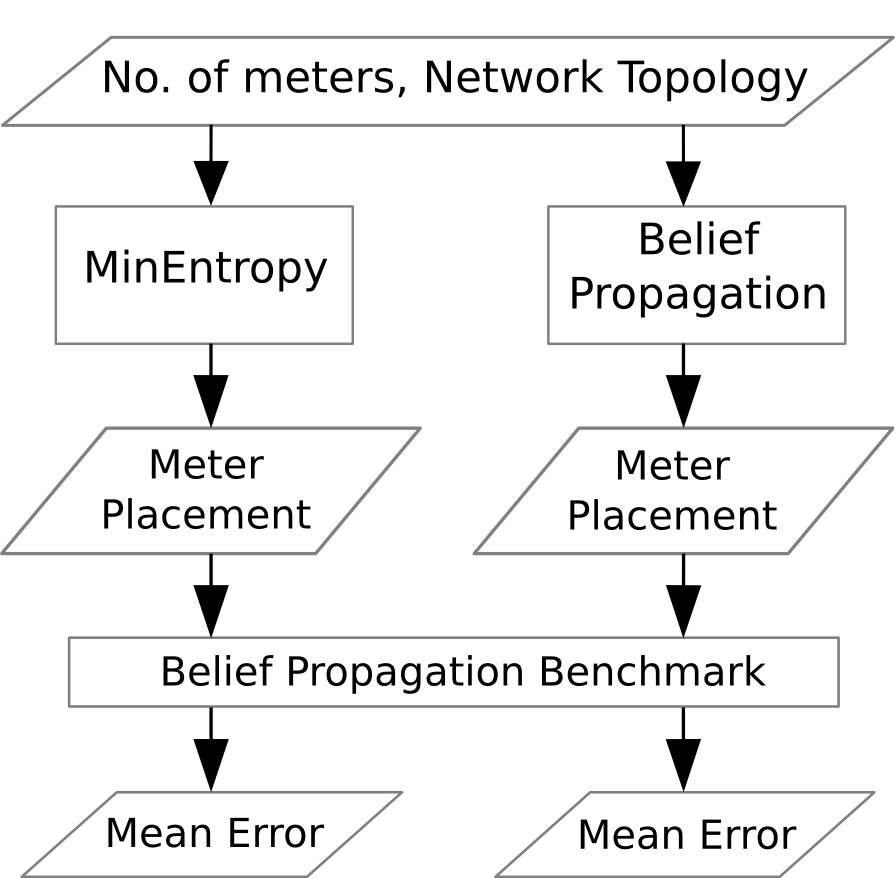
\includegraphics[width=0.55\textwidth]{benchmark}
\vspace{0.5cm}
\caption{An overview of the meter placement evaluation process. }
\label{fig:benchmark}
\vspace{2cm}
\end{figure}




\begin{figure}[!p]
\centering
\subfloat[Homogenous line network]{\label{Homogeneous line network}
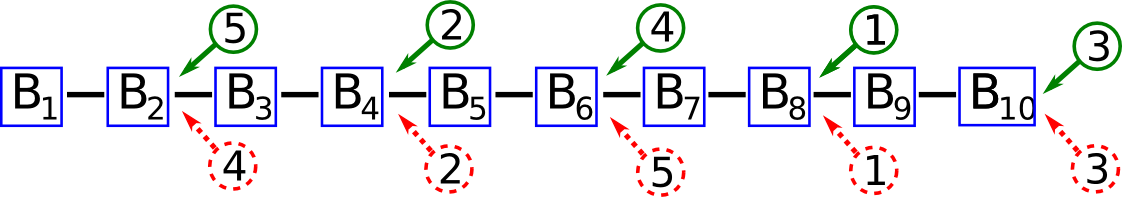
\includegraphics[width=0.68\columnwidth]{line_network_same}
}

\begin{centering}
\subfloat[Heterogeneous line network]{\label{HeterogeneousLineNetwork}
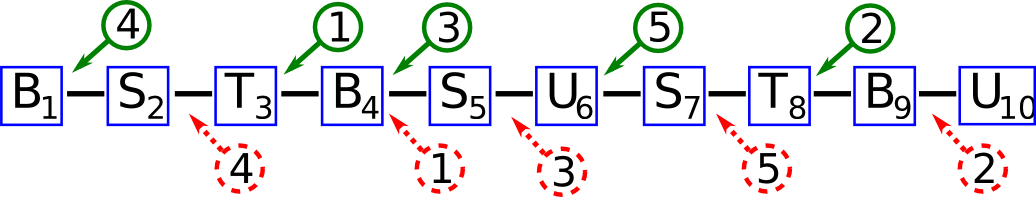
\includegraphics[width=0.65\columnwidth]{line_network_varied}
}
\end{centering}

\begin{centering}
\subfloat[Homogeneous tree network]{\label{HomogeneousTreeNetwork}
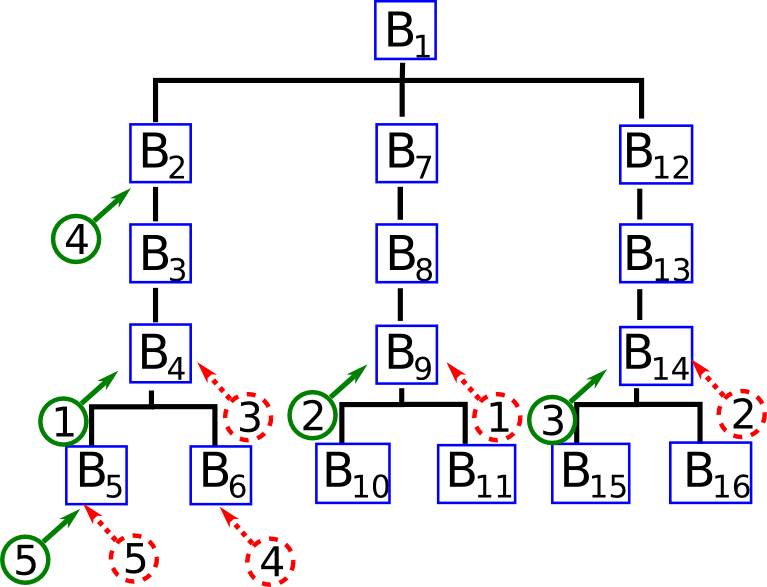
\includegraphics[width=0.45\columnwidth]{tree_network_same}
}
\subfloat[Heterogeneous tree network]{\label{HeterogenousTreeNetwork}
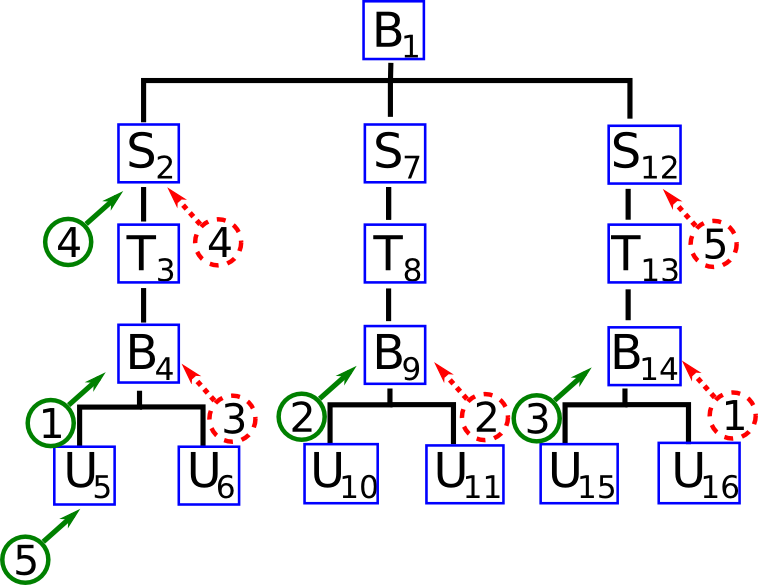
\includegraphics[width=0.45\columnwidth]{tree_network_varied}
}
\end{centering}

\begin{centering}
\subfloat[IEEE 13-node distribution test feeder network]{\label{13NodeTestFeederNetwork}
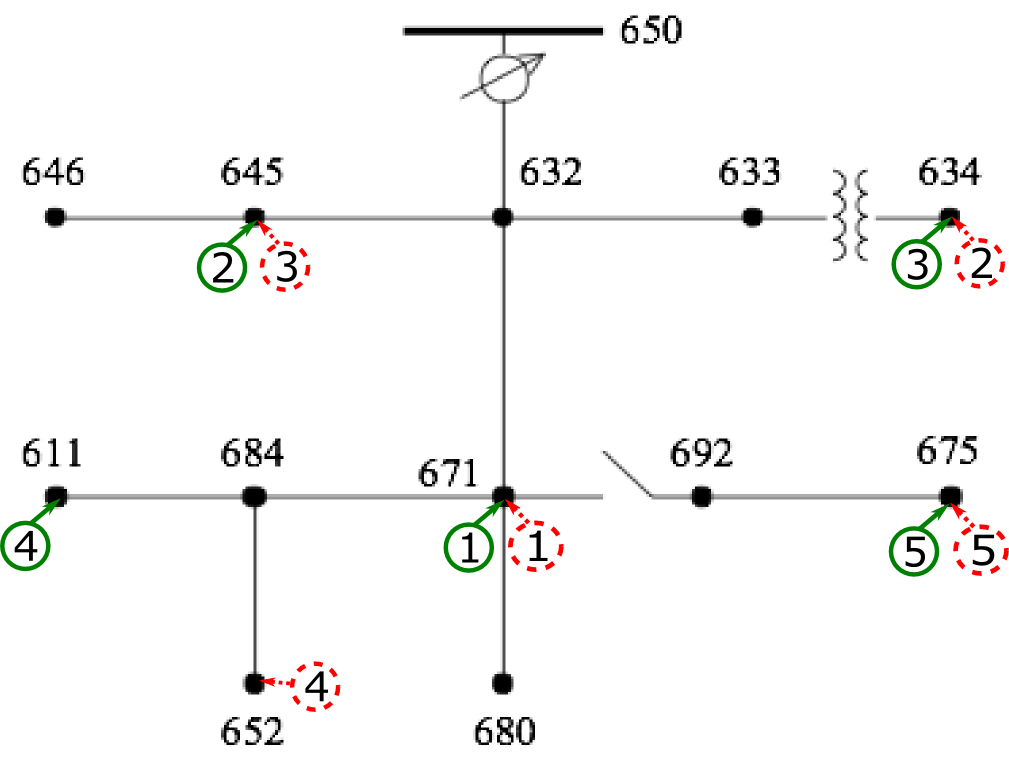
\includegraphics[width=0.6\columnwidth]{IEEE_13_node_test_feeder}
}
\end{centering}

\caption{Networks used in our experiments. B=bus, S=switch, T=transformer,
U=UPS. Ordered dotted circles correspond with the sequence of meters
placed by BP while the solid circles show the meter placed by MinEntropy.} 
\label{NetworkDiagrams}
%\vspace{-0.15in}
\end{figure}

Figure~\ref{NetworkDiagrams} shows the meters placed by the two algorithms in various network topologies. The positions of the meters placed by both algorithms are essentially similar. The MinEntropy algorithm achieves much faster results, completing in less than a second in all cases. On the other hand, the BP takes a longer time to complete. This is because BP compares individual samples on all links for every possible placement while the MinEntropy approach computes the conditional entropies at unmetered locations using probability mass functions instead of using individual samples. Algorithm completion times for both BP and CE approaches are shown in Table~\ref{network_configuration_results}.

\begin{table}[!p]
\vspace{1cm}
\renewcommand{\tabcolsep}{0.1 cm}
\renewcommand{\arraystretch}{1.8}
\centering
\caption{Results for each network configuration}
\label{network_configuration_results}
\begin{tabular}{|c|c|c|c|c|}
\hline \textbf{\thead{Network\\Topology}} & \textbf{Algorithm} & \textbf{\thead{Meter Placement \\ Sequence}} & \textbf{\thead{Mean \\ Error Rate}} & \textbf{\thead{Elapsed Time \\(seconds)}} \tabularnewline \hline 
\multirow{2}{*}{\thead{Line\\homogeneous}}& BP & 9,5,11,3,7 & 0.041112 & 270 \tabularnewline \cline{2-5}
& MinEnt & 9,5,11,7,3 & 0.041112 & 0.064 \tabularnewline \hline
\multirow{2}{*}{\thead{Line\\heterogeneous}}& BP & 5,10,6,3,8 & 0.040215 & 281 \tabularnewline \cline{2-5}
& MinEnt & 4,9,5,2,7 & 0.064040 & 0.064 \tabularnewline \hline 
\multirow{2}{*}{\thead{Tree\\homogeneous}}& BP & 10,15,5,7,6 & 0.057893 & 727 \tabularnewline \cline{2-5}
& MinEnt & 5,10,15,3,6 & 0.056891 & 0.138 \tabularnewline \hline 
\multirow{2}{*}{\thead{Tree\\heterogeneous}}& BP & 15,10,5,3,13 & 0.063510 & 727 \tabularnewline \cline{2-5}
& MinEnt & 5,10,15,3,6 & 0.071655 & 0.138 \tabularnewline \hline 
\multirow{2}{*}{\thead{IEEE 13-Node\\Test Feeder}}& BP & 671,634,645,652,675 & 0.052381  & 802  \tabularnewline \cline{2-5}
& MinEnt &  671,645,634,611,675 & 0.052381 & 0.138 \tabularnewline \hline 
\end{tabular}
\end{table}

\begin{table}[!p]
\renewcommand{\tabcolsep}{0.1 cm}
\renewcommand{\arraystretch}{1.4}
\centering
\caption{Number of meters required in various networks to restrict the mean error rate to 0.05 (5\%).}
%\vspace{-0.1in}
\label{cost_analysis}
\begin{tabular}{|c|c|c|c|c|c|}
\hline \textbf{Algorithm} & \textbf{\thead{Line\\Homogen.}} & \textbf{\thead{Line\\Heterogen.}} & \textbf{\thead{Tree\\Homogen.}} & \textbf{\thead{Tree\\Heterogen.}} & \textbf{\thead{IEEE 13-Node\\Test Feeder}} \tabularnewline \hline 
 BP     & 5 & 5 & 6 & 6 & 6 \tabularnewline \hline 
 MinEnt & 5 & 6 & 6 & 6 & 6 \tabularnewline \hline 
 \specialcell{Random} & 7 & 8 & 8 & 8 & 8 \tabularnewline \hline 
\end{tabular}
\vspace{2cm}
\end{table}

The meter placements are then passed to the belief propagation benchmark to compare the accuracy of the two algorithms in terms of mean-square error, i.e., the mean error between the estimated and actual transition functions on unmonitored links. We collect a set of known samples for a given meter configuration and infer the maximum likelihood power quality event that would appear at each unmetered node using belief propagation. We then estimate the error rate for each node. If the inferred event differs from the event given by the MC sample, we add $1/N$ for that sample. The mean error rate across all nodes is taken as the final performance metric. As shown in Table~\ref{network_configuration_results}, the MSEs are very small for both algorithms in all networks we tested. The BP algorithm gave slightly better estimations than MinEntropy in some cases at a cost of longer running times.

We also compare the accuracy of our algorithms in terms of cost savings. Table~\ref{cost_analysis} shows the number of meters needed by each algorithm where it can be clearly seen that using our solution to achieve the same accuracy (error rate of $< 0.05$) can reduce the number of meters by 33\%. Results of the Random placement algorithm were obtained by randomly placing meters until the desired accuracy was achieved.


\section{Conclusion}
\label{sec:conclusion}
Power quality meters are expensive devices and it is financially infeasible to install them on every link in the power network. We proposed algorithms which intelligently place power meters on selected power links to reduce the cost of power quality monitoring. We formulated the problem of selecting suitable meter placements in power networks such that power quality can be best predicted. Two approaches were presented, one based on conditional entropy and one considering prediction error. Experiments in various simulation networks including the IEEE 13-node distribution test feeder suggested that the conditional entropy-based MinEntropy approach is much faster. Finally, the proposed solutions significantly reduce the uncertainty of power quality values on unmonitored power links.